\chapter{Optimizing the performance of a centrifugal pump by data assimilation}



%En combien de temps l'information de pression remonte-t-elle dans le diffuseur ?


%144 coeurs : 54it/min
%300-> 336 coeurs : 100it/min (+- 20\%)

%– Le récit de l’expérience préprofessionnelle doit faire état de toutes les fonctions exercées par le stagiaire à son poste. Il doit comporter des développements techniques (illustrés par des schémas expliqués et commentés, par exemple), mais il s’agit avant tout de donner au lecteur une idée de ce que furent l’emploi du temps du stagiaire, ses tâches quotidiennes, les contraintes du métier, la nature des relations humaines dans cet environnement, les difficultés rencontrées et les résultats obtenus.
%– Les connaissances techniques acquises doivent transparaître dans le document. Le correcteur évaluera si celui-ci fait état d’une maîtrise réelle des outils (informatiques, mécaniques, etc.) utilisés pendant le stage. En outre, il estimera le niveau des connaissances techniques acquises que la rédaction du rapport aura su mettre en évidence.

The internship began in February 2025. I was provided with a fix computer, and credentials to connect to the Irene and Cassiopée supercomputers. Marcello MELDI, Antoine DAZIN and Miguel MARTINEZ VALERO which are my internship supervisors, showed me around the lab.
Then, Tom MOUSSIE and Miguel, my co-officies, explained to me the basics of OpenFoam and CONES, the DA code. I was able to run a few tests on OpenFoam on the supercomputers, which allowed me to familiarize myself with the tools and the code. % PARLER DE LA CONFIG DE CONES


% Introduction par thèse de Miguel

%Lors de mes essais sur le supercalculateur, j'ai utilisé une partition qui offre une puissance de calcul totale de 723 Tflop/s. Elle est composée de 185 nœuds Intel 2x18 cœurs Skylake, cadencés à 2,3 GHz avec 96 Go de mémoire. Ces ressources m'ont permis d'effectuer les tests demandant le plus de ressources.

\section{Data Assimilation}

% PAS d'equation ici, sinon je me fait frapper

DA\cite{aschDataAssimilationMethods2016} is a technique used to improve the accuracy of numerical models by combining them with observational data. It is widely used in various fields, including meteorology, oceanography, and engineering. The goal of data assimilation is to obtain a more accurate representation of the state of a system by integrating information from different physical measurements or hight fidelity sources. An illustration of the data assimilation process is shown in Figure \ref{fig:DAmap}.

% changer l'endroit de la citation

\begin{figure}[H]
    \centering
    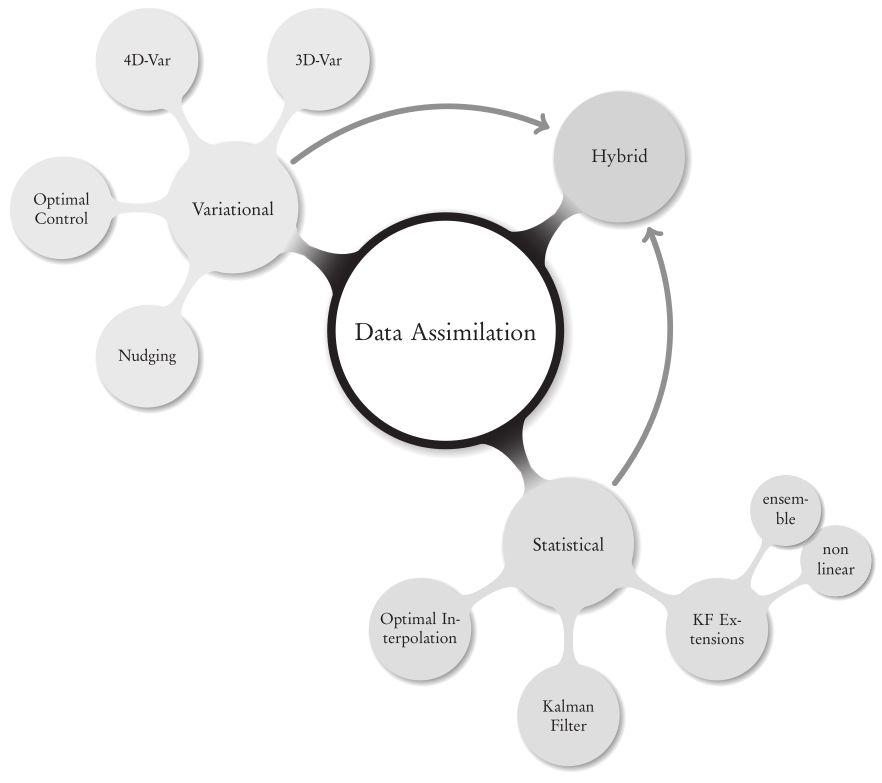
\includegraphics[width=0.60\textwidth]{images/other/DAmap.png}
    \caption{The big picture for DA methods and algorithms\cite{aschDataAssimilationMethods2016}}
    \label{fig:DAmap}
\end{figure}


\begin{figure}[H]
    \centering
    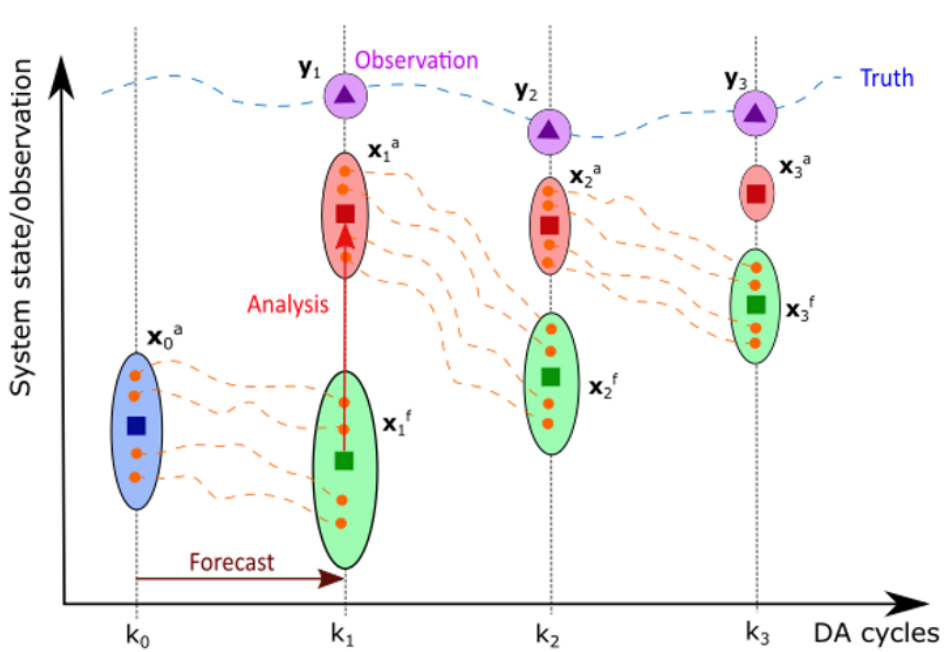
\includegraphics[width=0.60\textwidth]{images/enkf_shem.png}
    \caption{Illustration of the EnKF process (100\% confidence in observations)}
    \label{fig:EnKFIllustration}
\end{figure}


// Expliquer  théorème de Bayes etc... dans la partie maths (à ref ici)
%Expliquer plus en détail l'EnKF avec la fameuse figure.



\subsection{State of the art} % Introduction

\paragraph{EnKF} Our approach to data assimilation is based on the \ac{EnKF}, which is a Monte Carlo method that uses a set of model states (the ensemble) to estimate the state of the system. The EnKF is particularly well-suited for nonlinear systems and has been successfully applied in various fields, including computational fluid dynamics (CFD).

EnKF for DA in CFD has been used at LMFL since a few years, with the work of Lucas Villanueva\cite{villanuevaAugmentedStateEstimation2023}, Miguel M.Valero\cite{villanuevaAugmentedStateEstimation2023}, Tom Moussie\cite{moussieStatisticalInferenceUpstream2024a}, Sarp Er, Paolo Errante\cite{moussieStatisticalInferenceUpstream2024a} and Marcello Meldi\cite{villanuevaAugmentedStateEstimation2023}\cite{moussieStatisticalInferenceUpstream2024a} and his colleagues. The EnKF method is a powerful tool for assimilating data into computational fluid dynamics (CFD) simulations, allowing for the correction of model predictions based on observed data.



Today, we can theorically run a \ac{DNS} which resolves exactly the Navier-Stokes equations, but it is still too expensive to be used in practice. Therefore, we use \ac{LES} or \ac{RANS} models to simulate the flow. The EnKF method can be applied to these models to improve some of theme parameters or physical state, to improve the physical accuracy.

A good example based on the simple and academic \textit{cavity test case} illustrate it well.
The cavity test case is a simple flow in a square cavity, where the flow is driven by a moving lid. The flow is characterized by a recirculation zone and a vortex in the center of the cavity. The EnKF method can be used to assimilate data from the flow, such as velocity or pressure measurements, to improve the accuracy of the simulation. The EnKF method can also be used to estimate the parameters of the model, such as the viscosity or the turbulence model coefficients, to improve the physical accuracy of the simulation.
In our case, we are going to optimise the velocity wall condition.
For that, we use the result on 5 locations of a precise converged simulation with a to boundary condition of 5 m.s$^{-1}$ as a reference. We will then assimilate data from the flow, at the 5 observation points\ref{fig:cavity2_1ms}.
We start from a simulation with a wall condition of 1 m.s$^{-1}$, which is not the correct value. The EnKF method will then be used to correct the wall condition by assimilating the data from the flow at the 5 observation points. The EnKF method will iteratively update the wall condition until it converges to the correct value, which is 5 m.s$^{-1}$ in this case.

\begin{figure}[H]
    \centering
    \begin{subfigure}[b]{0.3\textwidth}
        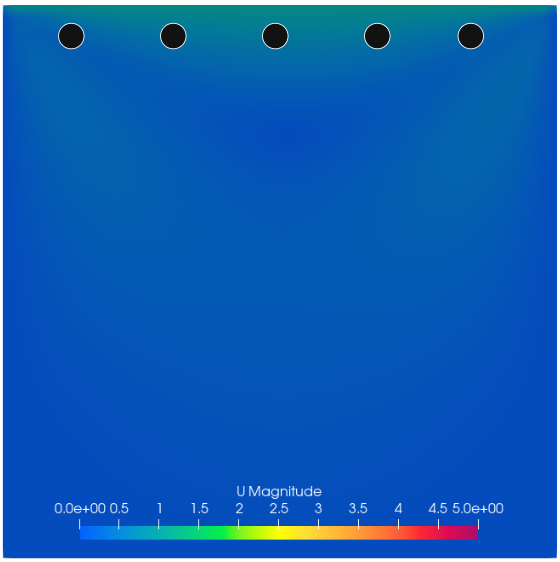
\includegraphics[width=\textwidth]{images/cavity/cavity3_1ms.png}
        \caption{Initial state}
        \label{fig:cavity2_1ms}
    \end{subfigure}
    \hfill
    \begin{subfigure}[b]{0.3\textwidth}
        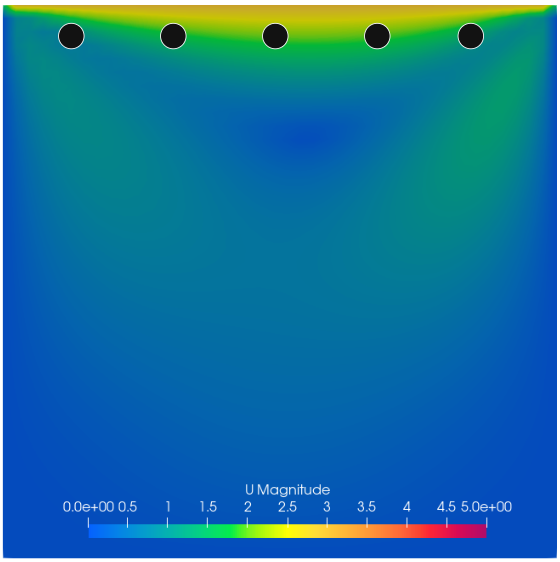
\includegraphics[width=\textwidth]{images/cavity/cavity3_3ms.png}
        \caption{After one EnKF it.}
        \label{fig:cavity2_3ms}
    \end{subfigure}
    \hfill
    \begin{subfigure}[b]{0.3\textwidth}
        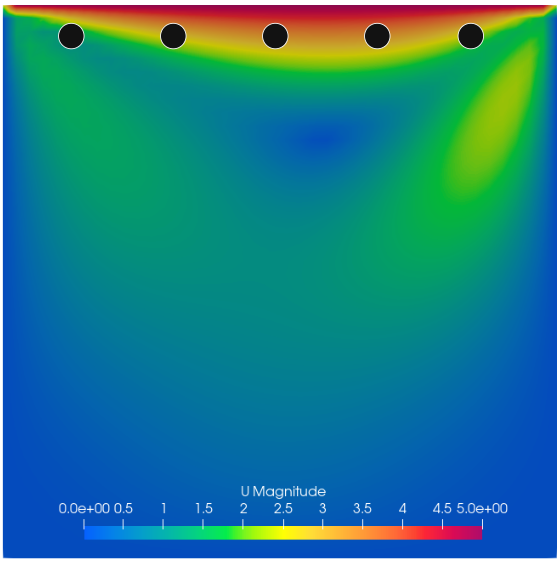
\includegraphics[width=\textwidth]{images/cavity/cavity3_5ms.png}
        \caption{Converged after 2 EnKF it.}
        \label{fig:cavity_5ms}
    \end{subfigure}
    \caption{Evolution of the state through EnKF iterations (
\includegraphics[width=0.014\textwidth]{images/cavity/legende.png}: observation point)}
\end{figure}




% Je cherche à transmettre quelle idée ?
% State of art : ce qui a été fait avant, ce qui est fait aujourd'hui, ce qui est fait dans le cadre de mon stage




\paragraph{IBM} The IBM theory has been developed in 1972 by Charles S. Peskin\cite{IBM_base}.
The Immersed Boundary Method (IBM) is a numerical technique used to simulate fluid-structure interactions, particularly in cases where the structure is immersed in a fluid flow. It permit to keep numerical precision on complex geometries and moving boundaries without the need for body-fitted meshes, which can be computationally expensive and difficult to implement.

They are differents ways to discretize the space when we do CFD (see Figure \ref{fig:solidworksMesh}\footnote{\url{https://www.solidworks.com/sw/docs/flow_basis_of_cad_embedded_cfd_whitepaper.pdf}}). The most common are structured meshes, unstructured meshes and body-fitted meshes. The body-fitted meshes are the most accurate but also the most expensive in terms of computational resources. The IBM allows to use unstructured meshes, which are less accurate but more efficient in terms of computational resources.

\begin{figure}[H]
    \centering
    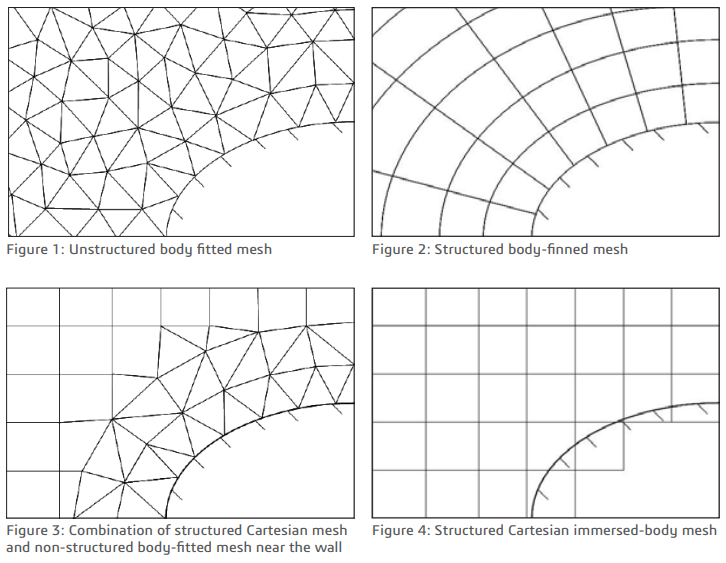
\includegraphics[width=0.8\textwidth]{images/solidworksMesh.png}
    \caption{Differents ways to mesh}
    \label{fig:solidworksMesh}
\end{figure}


In our case, we impose a forcing term on the Navier-Stokes equations to simulate the effect of the immersed boundary on the fluid flow. // ref à plus tard. The problem is that it it lead to a few constants that need to be tuned to obtain the best results. For that, we use the EnKF method to optimize these constants. The EnKF method will be used to assimilate data from the flow at the observation points and to update the forcing term until it converges to the optimal value.

These high fidelity data are obtained from an experiment explained in the next subsection
\begin{figure}[H]
    \centering
    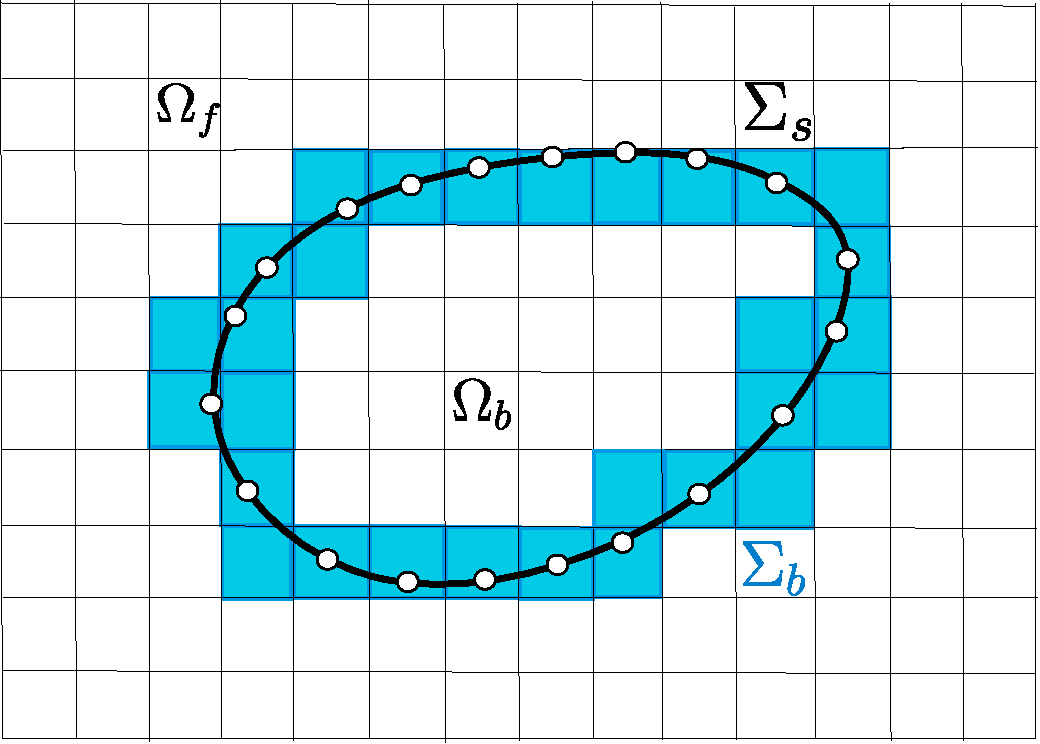
\includegraphics[width=0.45\textwidth]{images/IBM_Mesh.pdf}
    \caption{...}
    \label{fig:IBM_Mesh}
\end{figure}
Quel niveau de détail ici ?

% DONE (aller de + en plus en détail jusqu'a param IBM car gros cas test couteux en body-fitted)

This year, my supervisors M. VELRO and M. Meldi published an article\cite{valero2025immersed} about the optimisation of the IBM forcing and turbulence terms, that gives very good results. More recently, they obtain very good results on the optimisation of this parameters on a ascillating cylinder. // Tt ça à vérifier en relisant la thèse de Miguel.

% DONE Et là cas tests de thèse miguel (1 et 2)

This lead us to the idea of using the EnKF method to optimize the parameters of the IBM forcing term on a centrifugal pump, which is a more complex case than the previous ones. The goal is to improve the performance of the pump by optimizing the parameters of the IBM forcing term, which will lead to a better simulation of the fluid flow and a better understanding of the pump's behaviour.

% Puis amener cas 3 (pompe) pour transitionnre vers la sous-parite suivante

\subsection{Presentation of the test case: the centrifugal pump}


Parler rapidement qu'on a des données (pression et PIV)

Centrifugal pumps are used since 1475\cite{retiFrancescoDiGiorgio1963} and are still widely used today in various applications, such as water supply, irrigation, turbomachines, and industrial processes. They are known for their low cost, efficiency and reliability, making them a popular choice for many fluid transport applications.

\begin{figure}[H]
    \centering
    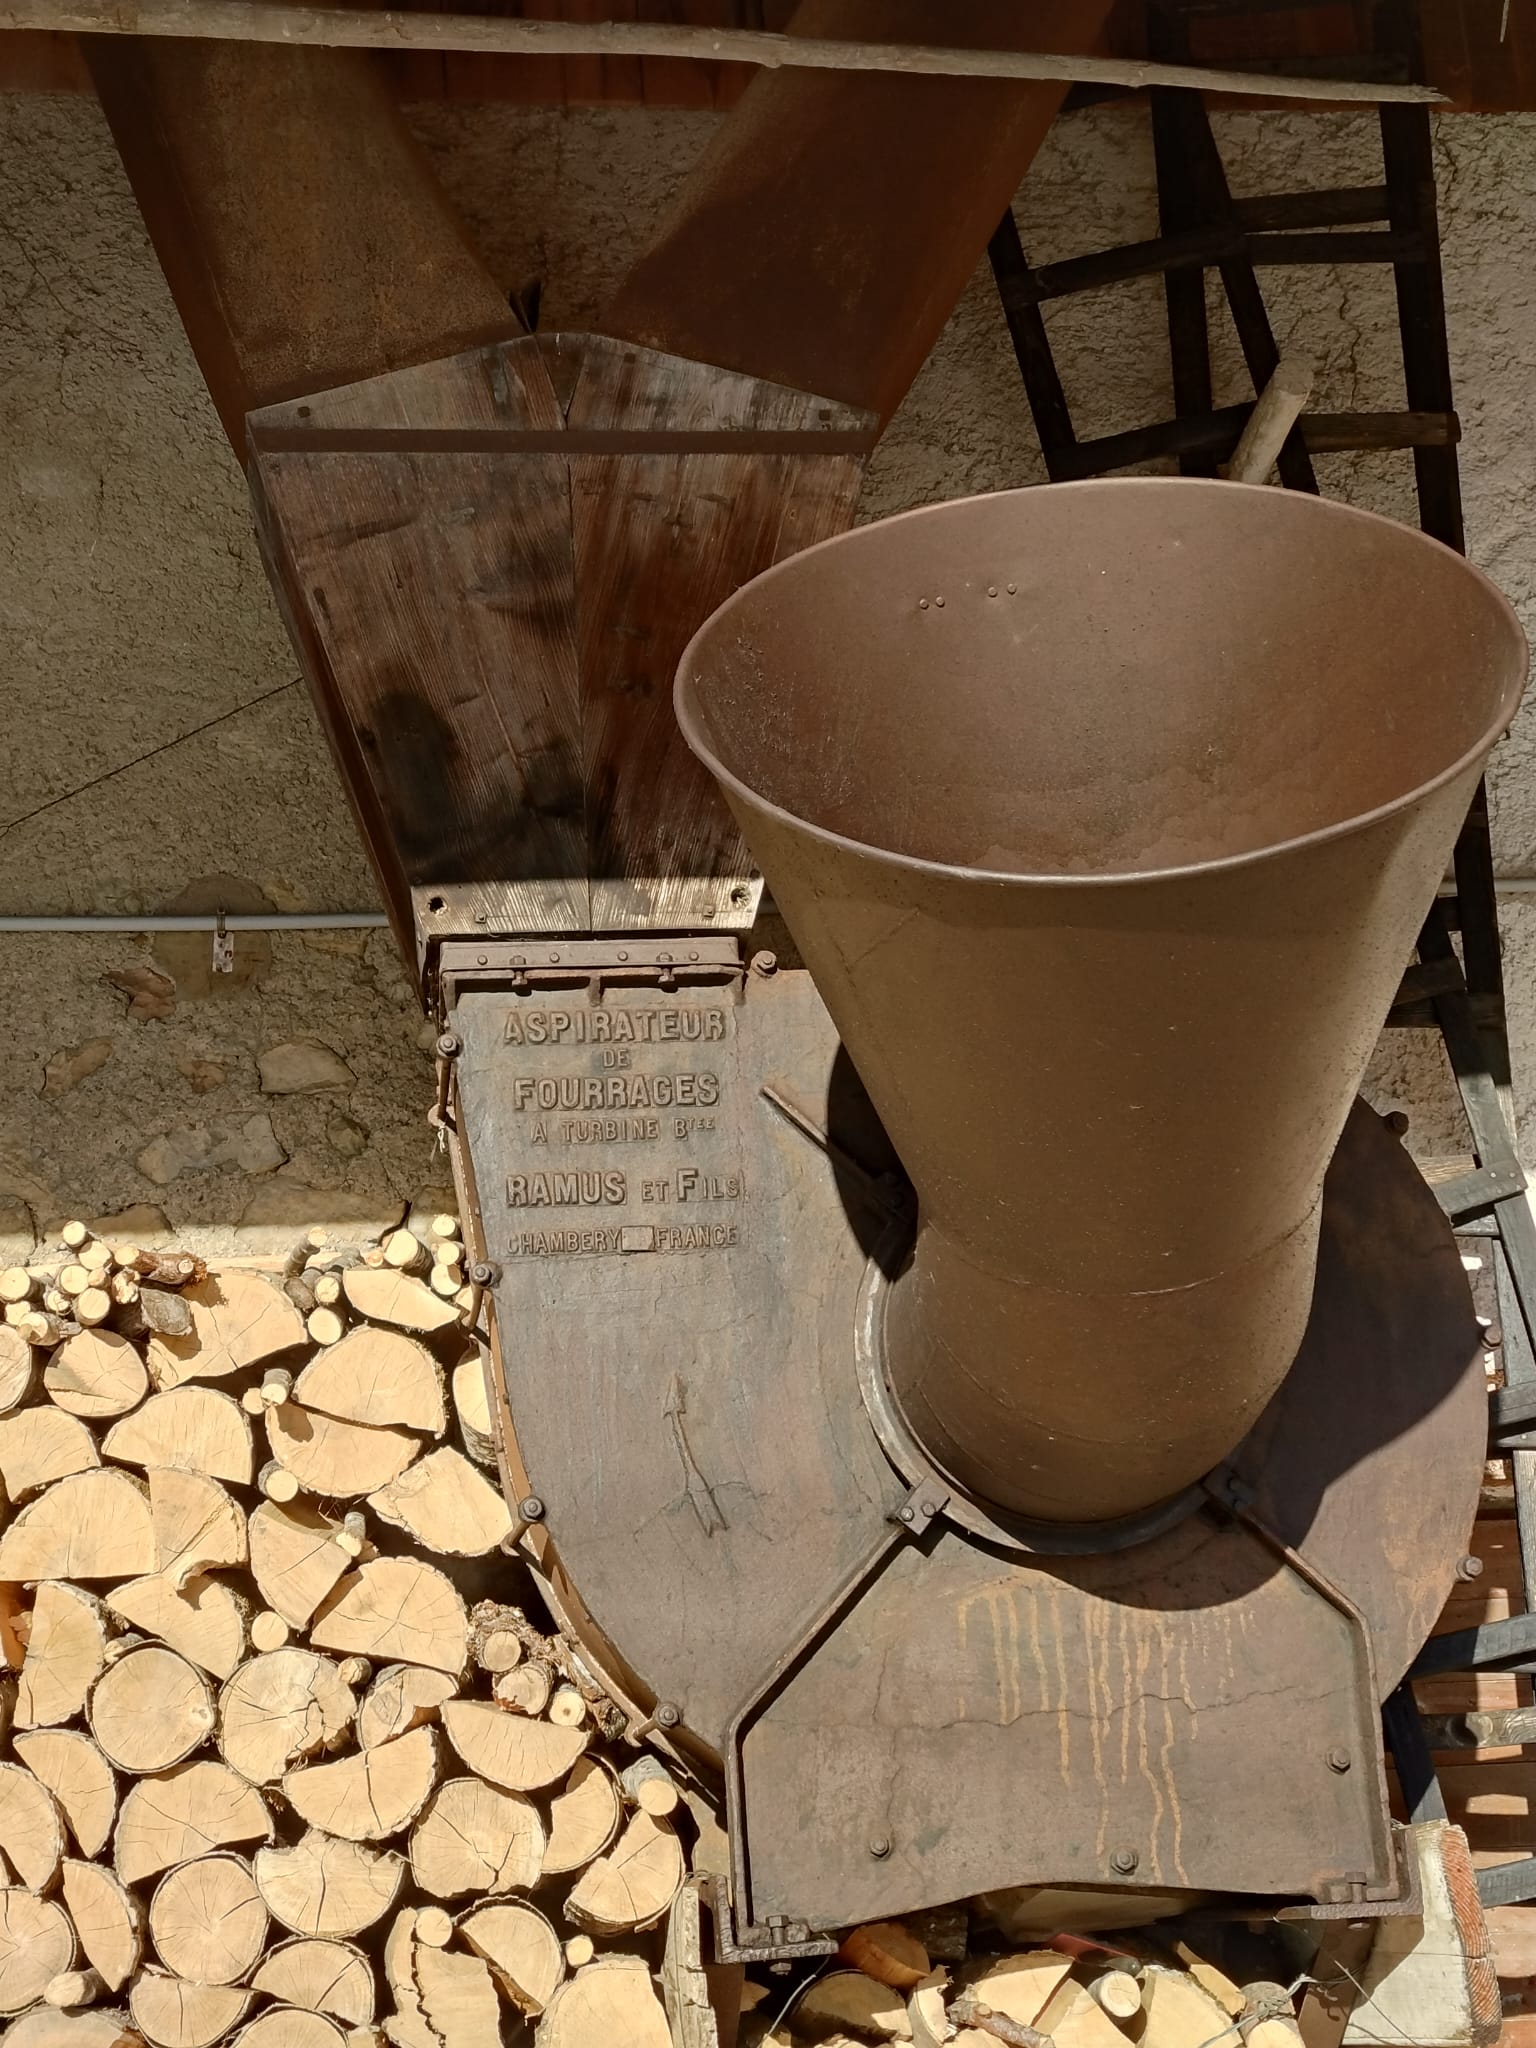
\includegraphics[width=0.40\textwidth]{images/other/pompe_centrifuge.jpg}
    \caption{Old centrifugal pump used to move hay (personnal picture)}
    \label{fig:old_centrifugal_pump}
\end{figure}


The studied centrifugal pump is a SHF impeller, which is a type of centrifugal pump designed for high flow rates and low head applications.
These high fidelity data are obtained from an experiment realised by Antoine Dazin\cite{dazinHighspeedStereoscopicPIV2011a} in 2011 at the LMFL. The experiment was realised on the SHF impeller on the RESEDA centrifugal pump benchmark. -> a vérifier dans la thèse de Miguel
% PARLER

Results in the file are High-Speed \ac{PIV} data obtained by Antoine DAZIN in 2011\cite{dazinHighspeedStereoscopicPIV2011a} at a PIV frequency of 980 Hz on a SHF impeller % Expliquer la PIV ?
The operating conditions of the machine where :

\begin{table}[!h]
    \centering
    \begin{tabular}{c c c}
        \multicolumn{3}{c}{\textbf{Impeller characteristics}} \\ \hline 
         $R_1$ & Tip inlet radius & $141.1\,mm$  \\
         $R_2$ & Outlet radius & $257.5\,mm$ \\ 
         $Z$ & Number of blades & $7$ \\
         $Q_d$ & Design flow rate & $0.236\,m^3/s$ \\ % 0.256 ???
         $K$ & Mean blade thickness & $9\,mm$ \\
         $\Omega$ & Rotating velocity & $1\,200\,rpm$ \\ 
         $\beta_2$ & Outside blade angle (from peripheral velocity $U=R_2\Omega$) & $22.5^{\circ}$ \\ \hline \hline
        \multicolumn{3}{c}{\textbf{Vaneless diffuser characteristics}} \\ \hline
         $b_3$ & Diffuser width & $38.5\,mm$ \\
         $R_3$ & Inlet radius (without leakage, i.e., $R_3=R_2$) & $257.5\,mm$ \\
         $R_4$ & Diffuser outlet radius & $385.5\,mm$ \\
         $t$ & Thickness of the upper and lower sections of the diffuser & $20\,mm$
    \end{tabular}
    \caption{Summary of the main geometrical and operating parameters of the impeller and diffuser at design conditions, employed in the numerical modelling of the centrifugal pump.}
    \label{tab:pump_parameters}
\end{table}


\begin{figure}[H]
    \centering
    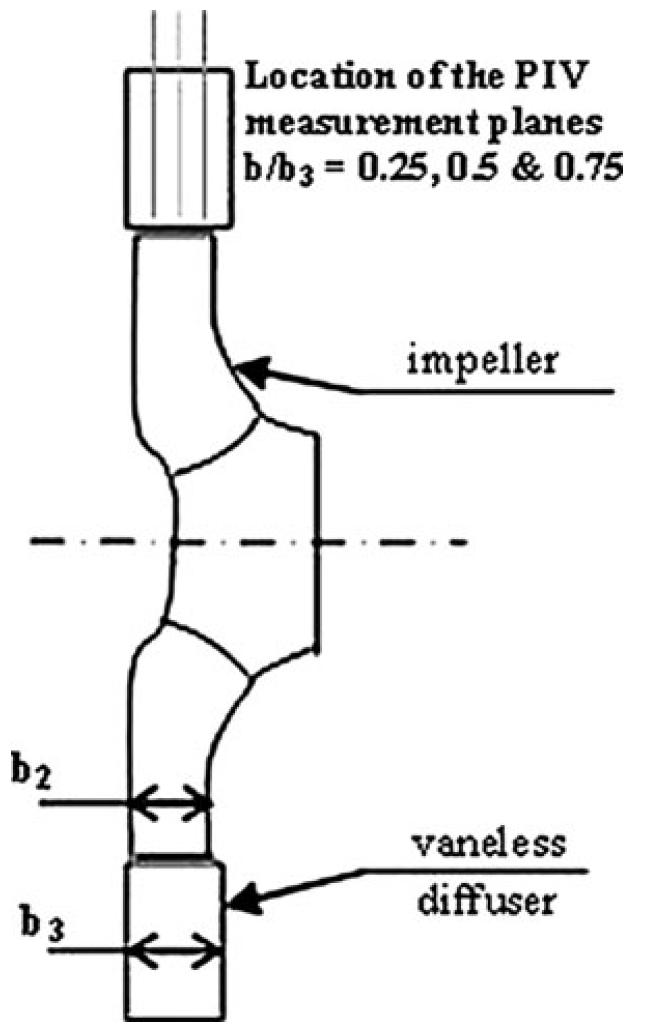
\includegraphics[width=0.4\textwidth]{images/experimentalPump/impeller_position.png}
    \caption{Position of the PIV plans}
    \label{fig:PIVPlans}
\end{figure}

The data is stored in a directory structure that contains 6 directories
The 6 directories are corresponding to two tests realised at 25\%, 50\% et 75\% of the diffuser height.
Each test was repeated twice for the same operating condition and the same height (R1, R2)
In each directory, there are 1581 files corresponding to instantaneous ASCII data file.
The 9 columns are corrresponding to :

%centrer
$x(m),y(m),V_x(m.s^{-1}),V_y(m.s^{-1}),r(m),\theta(rad),Vr(m.s^{-1}),V_{\theta}(m.s^{-1}),V_z(m.s^{-1}),\textit{Unknown}$

%The pdf is a paper where can be found the experimental conditions even if the analysis are focussed on another flow rate.

The theorical average speed at the input of the diffuseur is equal to \[\frac{Q_{dif_{in}}}{S_{dif_{in}}} = \frac{Q_{pump_{in}}}{2\pi R_{3} h_{dif}} = 3.65m.s^{-1}\]
With $Q_{pump_{in}} = Q_{dif_{in}}$ because the mass flow rate is constant and the flow is incompressible.

%Détail : R3 = 0.257m; h=0.0400m; Q = 0.236m3/s -> S=0.0646m2

\title{Fonctionning}  % ????
\title{Utility}


%Données hautes fidélités,...


\section{Numerical ingredients}

\subsection{CFD governing equations}



\begin{equation}
    (\boldsymbol{u} \cdot \boldsymbol{\nabla})\, \boldsymbol{u} = 
    -\frac{1}{\rho} \nabla p + \nu \nabla^2 \boldsymbol{u} 
    \underbrace{- \xi \nu \boldsymbol{D} \left( \boldsymbol{u} - \boldsymbol{u}_{ib} \right)}_{\boldsymbol{f}_P}
\end{equation}



with $[p] = M \cdot L^{-1} \cdot T^{-2}$ 
(formalisme divisé par la masse volumique $\rho$. Donc $[\boldsymbol{u}] = L \cdot T^{-1}$ - en incompressible).

\begin{equation}
    \xi = \left\{
    \begin{array}{ll}
        0 & \textrm{if } \boldsymbol{x} \in \Omega_f \\
        1 & \textrm{if } \boldsymbol{x} \in (\Sigma_b \cup \Omega_b)
    \end{array} \right.
\end{equation}

see Figure \ref{fig:IBM_Mesh}

When  $D \rightarrow \infty$, problèmes
        
mais des valeurs trop élevées de $D$ peut mener à des instabilités <- A mentionner qqpart 




Fluid mechanics is governed by the NS equations :




- Equations (Incompressible, turbulence,...)
- Ajout IBM\ref{fig:IBM_Mesh} -> Methodo (forcage continue ici (vs interpolation ?)) -> avantages
- Ajout MRF

% A écrire à ma facon, juste équations intéréssantes ici
Darcy's law in the body interface region $\Sigma_b$ and the solid region $\Omega_b$. To do so, a spatial dependent tensor $\boldsymbol{D}(\boldsymbol{x})$ must be defined. The resulting penalty term is modelled as follows:

\begin{equation}
     \boldsymbol{f}_P = \left\{
        \begin{array}{ll}
        \boldsymbol{0} & \textrm{if } \boldsymbol{x} \in \Omega_f \\
        -\nu \, \boldsymbol{D} \left(\boldsymbol{u} - \boldsymbol{u_{ib}} \right) & \textrm{if } \boldsymbol{x} \in (\Sigma_b \cup \Omega_b)
        \end{array} \right.
    \label{eqn:forcePenDarcy}
\end{equation}
$\boldsymbol{u_{ib}}(\boldsymbol{x}, t)$ is a target velocity representing the immersed body's physical behaviour. ... $\boldsymbol{u_{ib}}=\boldsymbol{0}$. The components $D_{ij}$ of the tensor $\boldsymbol{D}$ are usually controlled to obtain the best compromise between the accuracy and stability of the numerical solver %\cite{Verzicco2022_arfm}. The choice performed is crucial in the proximity of the grid transition between the fluid $\Omega_f$ and the interface $\Sigma_b$ regions.

$Re_\Omega=\cfrac{R_2^2 \Omega}{\nu} = 5.53\times10^5$ 

$Ma = \cfrac{R_2 \Omega}{c} = 0.095$ \textrm{\textbf{(incompressible)}}

Reprendre ma présentation (dimensiosn de p)

\begin{equation*}
    \boldsymbol{\nabla} \cdot (\boldsymbol{u}\boldsymbol{u}) = -\nabla p + \nu \nabla^2 \boldsymbol{u}  \overbrace{-\frac{\xi}{\eta} \left(\boldsymbol{u} - \boldsymbol{u_{ib}} \right)}^{\boldsymbol{f}_P}
\end{equation*}

\begin{equation*}
    \xi = \left\{
   \begin{array}{ll}
   0 & \textrm{if } \boldsymbol{x} \in \Omega_f \\
   1 & \textrm{if } \boldsymbol{x} \in (\Sigma_b \cup \Omega_b)
   \end{array} \right.
\end{equation*}

\subsection{The open source code OpenFoam}

To implemente the IBM forcage, we use the open source code OpenFoam, which is a C++ library for computational fluid dynamics (CFD). OpenFoam provides a wide range of tools for solving the Navier-Stokes equations, including solvers, meshing tools, and post-processing tools. It is widely used in the CFD community and has a large user base.

More precisely, for example, to implemente the IBM forcage on the speed U, we compute the forcing term $\boldsymbol{f}_P$ as follows:
\begin{lstlisting}[language=C++]
// Compute the forcing term
volVectorField fP = -fP_ * (U - U_ib); EXEMPLE DE MISE EN FORME A CORRIGER
// Add the forcing term to the momentum equation
U += fP;
\end{lstlisting}

\begin{figure}[H]
    \centering
    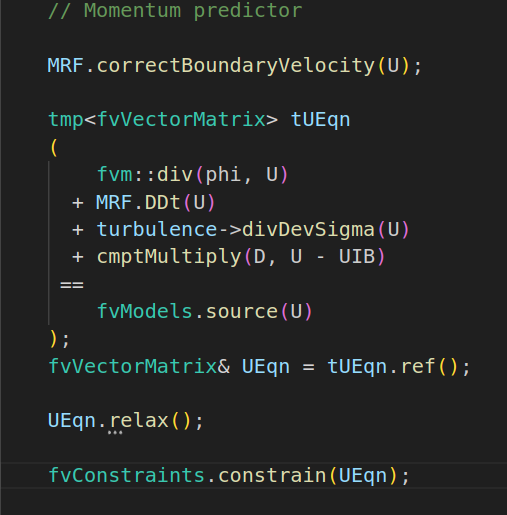
\includegraphics[width=0.5\textwidth]{images/other/implicit_forcing.png}
    \caption{implicit forcing term in OpenFoam}
    \label{implicit_forcing}
\end{figure}




To compute the time step $\Delta_{t}$ of the pimpleFoam simulation of the pump, we can use the \ac{CFL} condition, which states that:
\begin{equation}
    \Delta_{t} = \frac{CFL \cdot \Delta_{x}}{\|U_{\infty}\|},
\end{equation}
where:

- $CFL$ is the Courant number, typically set to 0.5 for stability. A way to visualize this is to think of it as the fraction of the distance a wave travels in one time step relative to the distance between two cells in the azimuthal direction at the tip of the impeller.
- $\Delta_{x}$ is the distance between two cells in the azimuthal direction at the tip of the impeller in our model, which is given as 1.5 mm or 0.0015 m.
- $\|U_{\infty}\|$ is the magnitude of the velocity at infinity, which can be approximated by the tangential velocity at the tip of the impeller.
\begin{equation}
    \|U_{\infty}\| = \omega \cdot r_{tip}
\end{equation}
where:
- $\omega$ is the angular velocity in radians per second,
- $r$ is the radius at the tip of the impeller.
Assuming the rotating speed is given in revolutions per minute (rpm), we can convert it to radians per second:
\begin{equation}
    \omega = \frac{1200 \text{ rpm} \cdot 2\pi \text{ rad}}{60 \text{ s}} = 125.66 \text{ rps}.
\end{equation}
Assuming the radius at the tip of the impeller is $r = 0.2566 \text{ m}$ (which is 0.2566m), we can compute the tangential velocity:
\begin{equation}
    \|U_{\infty}\| = 125.66 \text{ rps} \cdot 0.2566 \text{ m} =  \text{32.24 m/s}.
\end{equation}
Assuming the distance between two cells in the azimuthal direction at the tip of the impeller is $\Delta_{x} = 0.0015 \text{ m}$ (which is 1.5 mm), we can now compute the time step $\Delta_{t}$:
\begin{equation}
    \Delta_{t} = \frac{0.5 \cdot 0.0015 \text{ m}}{32.24 \text{ m/s}} = 2.3 \times 10^{-5} \text{ s} % \approx 2.3 \mu s.
\end{equation}


\subsection{EnKF}

Toujours mentionner les paramètres utilisés (dans le controlDict et le CONESDict)

\subsection{The library CONES}
CONES is a library coded in Python/C++ developed for ... since 2022 at LMFL. -> appuyer sur "seule online pour CFD à la connaissance du labo"
It's parallelized and can be used on supercomputers. It is mainly designed to work with OpenFoam and DA codes as EnKF.\label{instants_partages}

Simulations are performed using the C++ framework OpenFOAM, used to discretize the equations previously presented. Standing for \textsl{Open Source Field Operation and Manipulation}, OpenFOAM is an open-source which provides many tools, referred to as executables %\citep[see][]{greenshields2021}. These executable files can be divided into three separate categories:
\begin{itemize}
    \item[$-$] \textbf{Pre-processing}, including meshing and decomposing tools.
    \item[$-$] \textbf{Solving}, including in-built and custom solvers. Each solver is built to answer a specific CFD problem. 
    \item[$-$] \textbf{Post-processing}, including \texttt{ParaView}, an open-source visualization application.
\end{itemize}

OpenFOAM is not provided with a graphical interface, which is why a simulation is built by writing ``dictionaries'', in which are stored the necessary information for the simulation (mesh, turbulence model, maximum number of characteristic times, $\dots$). Thus, a specific directory structure must be observed, as outlined in ... % \autoref{fig:OpenFOAM_directory_structure}:
% décrire la structure du dossier OpenFOAM et ce que chaque fichier fait (dans mon cas de simulation)

\begin{figure}[H]
    \centering
    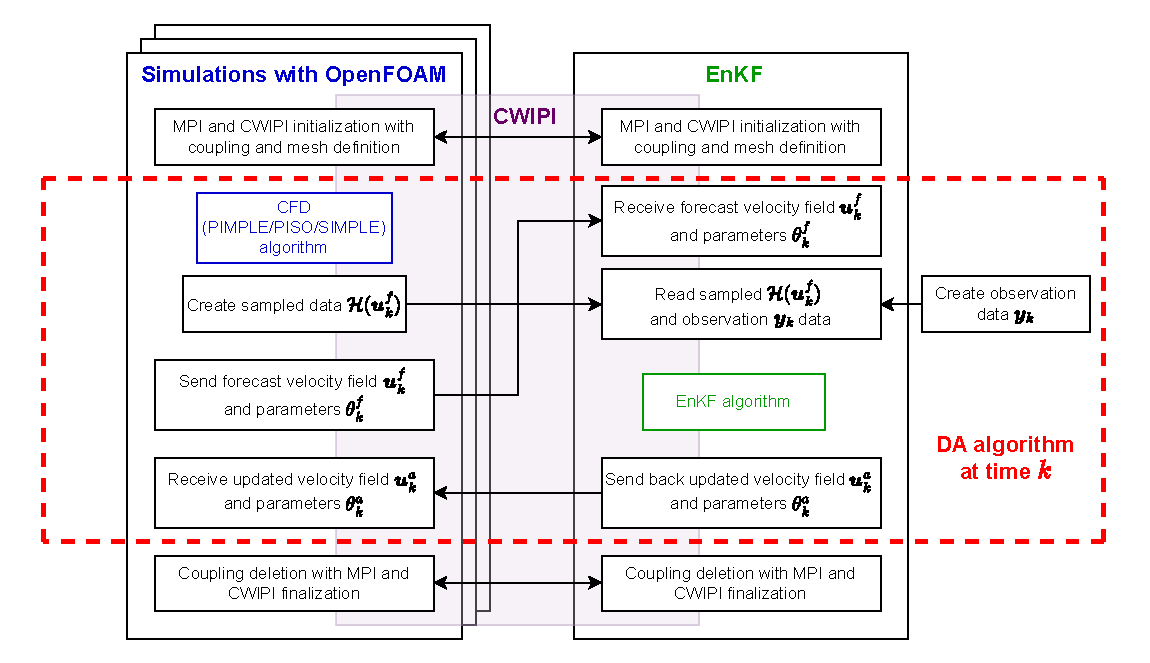
\includegraphics[width=0.5\textwidth]{images/EnKF_Cones.pdf}
    \caption{Model}
    \label{model}
\end{figure}


\begin{forest}
    for tree={
      font=\ttfamily,
      grow'=0,
      child anchor=west,
      parent anchor=south,
      anchor=west,
      calign=first,
      inner xsep=7pt,
      edge path={
        \noexpand\path [draw, \forestoption{edge}]
        (!u.south west) +(7.5pt,0) |- (.child anchor) pic {folder} \forestoption{edge label};
      },
      before typesetting nodes={
        if n=1
          {insert before={[,phantom]}}
          {}
      },
      fit=band,
      before computing xy={l=15pt},
    }  
  [root
    [system
      [controlDict
      ]
      [blockMeshDict
      ]
      [decomposeParDict
      ]
      [fvSchemes
      ]
      [fvSolution
      ]
    ]
    [templates
    ]
    [tests
    ]
  ]
  \end{forest}



\begin{figure}[H]
    \centering
    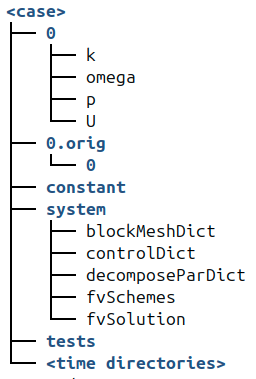
\includegraphics[width=0.3\textwidth]{images/other/OF_arbo.png}
    \caption{Arbo of OpenFoam}
    \label{arboOF}
\end{figure}


The \texttt{system} directory contains the main parameters concerning the progress of the simulation:
\begin{itemize}
    \item[$-$] The \texttt{controlDict} dictionary defines parameters such as start and end time, time steps, data output formatting, or data average computation.
    \item[$-$] The \texttt{blockMeshDict} dictionary defines the geometry, mesh and boundary conditions implementation.
    \item[$-$] The \texttt{decomposeParDict} dictionary defines the geometry and mesh decomposition, with the objective to run the simulation in parallel, using multiple cores.
    \item[$-$] The \texttt{fvSchemes} dictionary defines the discretisation schemes used in the solution.
    \item[$-$] The \texttt{fvSolution} dictionary defines the equation solvers, tolerances and other algorithm controls for instance. 
\end{itemize}

The \texttt{constant} directory contains the different physical properties of the simulation. Moreover, the subfolder \texttt{polyMesh} contains the mesh data, obtained after the \texttt{blockMesh} command line is run:
\begin{itemize}
    \item[$-$] The \texttt{momentumTransport} dictionary defines the simulation type (\ac{RANS} or \ac{LES}), as well as the turbulence model.
    \item[$-$] The \texttt{transportProperties} dictionary defines the transport model (Newtonian for instance) and some transport coefficients, such as the kinematic viscosity $\nu$. 
    \item[$-$] The \texttt{turbulenceProperties} dictionary defines the different parameters of the chosen turbulence model.
\end{itemize}

The \texttt{0} directory contains the initial solution's fields. The \texttt{postProcessing} directory stores data from the running simulation, such as forces and probes' data. The \texttt{processor0...N} directories directly result from the geometry decomposition, which is proceeded through the \texttt{decomposeParDict} dictionary. The \texttt{dummy.foam} is an empty file which allows to visualize the simulation with \texttt{ParaView}. 


\subsection{Pump modeling}

The objective of the model is to try to find same physical behavior as the experimental data. We call that digital twin.

For that we have first to discretize the numerical model of the pump. The mesh is generated using the \texttt{blockMesh} utility, which is a built-in OpenFOAM tool. The mesh is composed of 12 million cells. The mesh is composed of hexahedral cells. (quasi only, exepted some interface, cf figure). We don't need complex mesh because we dont neek to fit the geometry of the impeller.

Boundary conditions are defines as that:
\begin{itemize}
    \item[$-$] Inlet: velocity inlet
    \item[$-$] Outlet: pressure outlet
    \item[$-$] Wall: no-slip wall
\end{itemize}


\begin{figure}[H]
    \centering
    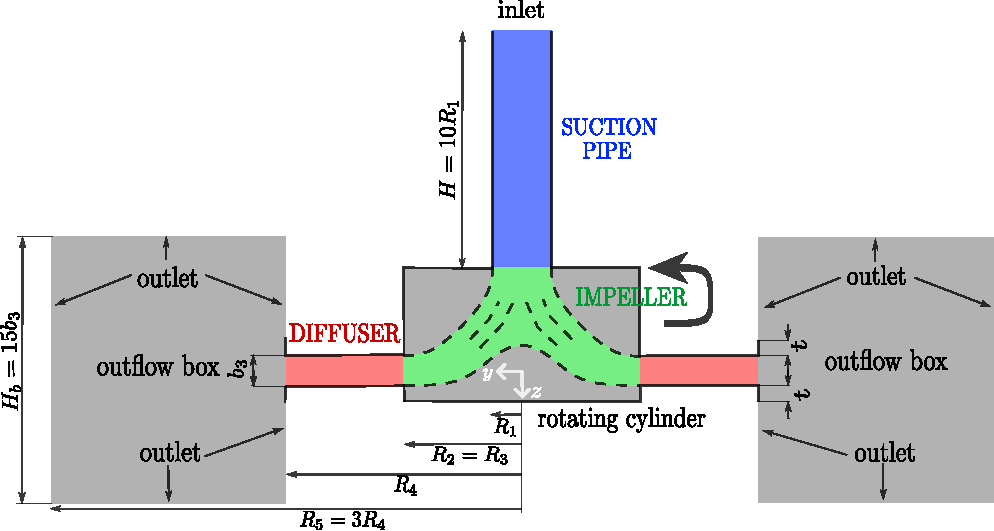
\includegraphics[width=0.5\textwidth]{images/model/RESEDA_sketch.pdf}
    \caption{Model}
    \label{Model}
\end{figure}

\section{IBM preliminary results}

"Résultats de la simulation avec 3e5" -> 3e7





Graçe aux données xp (mentionné partie 2.1.2, on peut faire d la DA)



\begin{figure}[H]
    \centering
    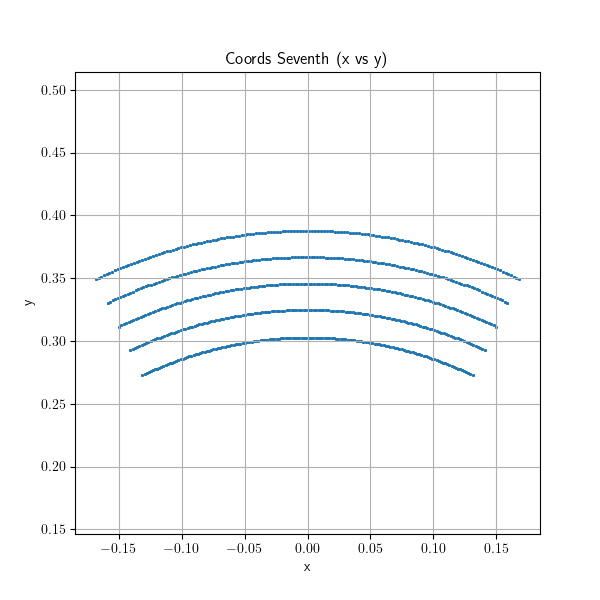
\includegraphics[width=0.5\textwidth]{images/coordsSeventh.png}
    \caption{Interpolation points over 360/7 degrees}
    \label{coordsSeventh}
\end{figure}


Notre but : faire fit ces 2 courbes : 

\begin{figure}[H]
    \centering
    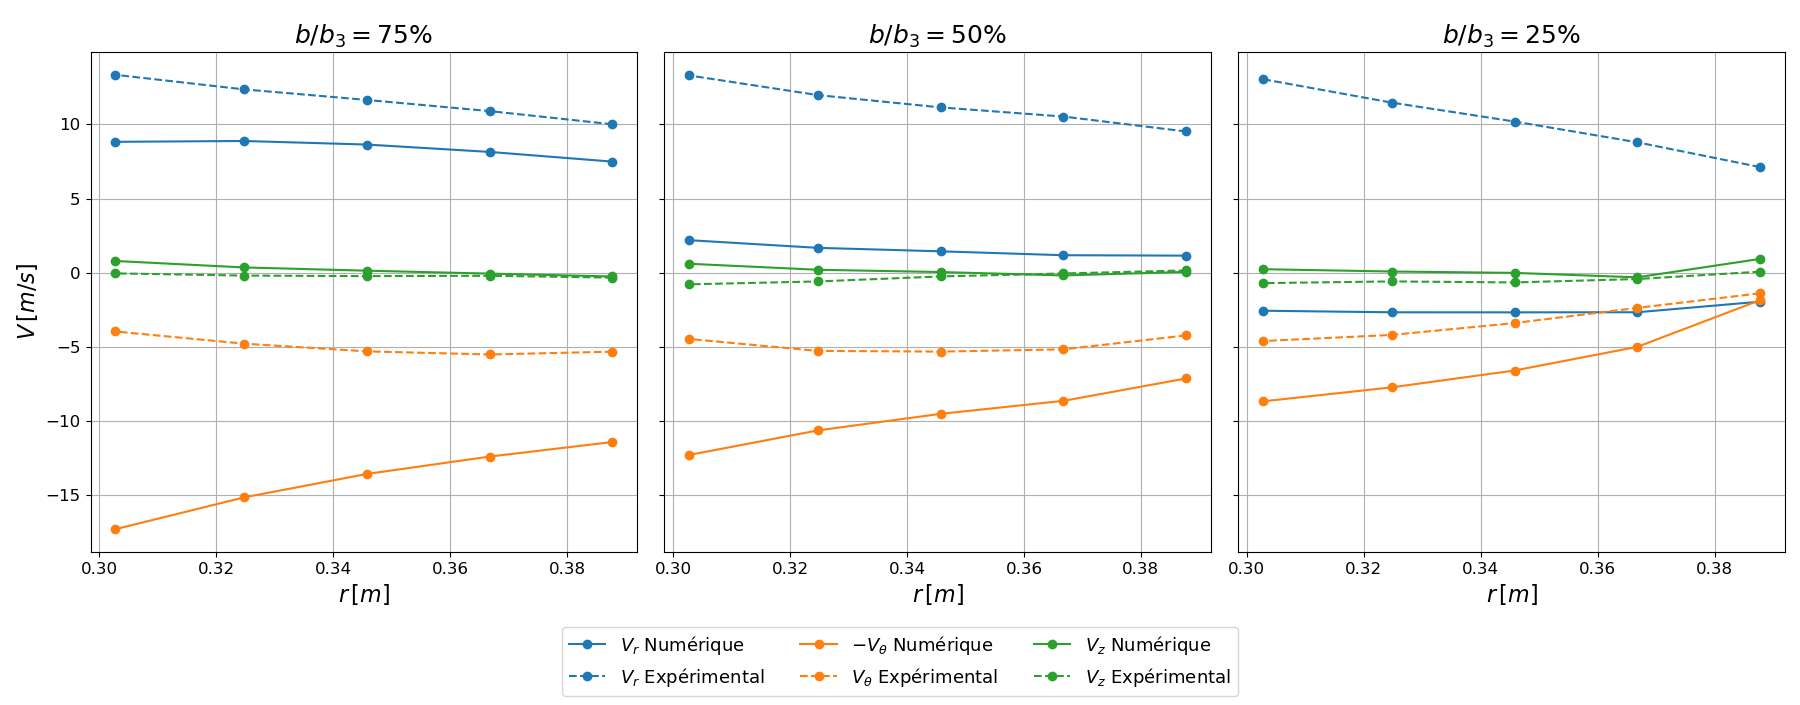
\includegraphics[width=1\textwidth]{images/numVSxp.png}
    \caption{implicit forcing term in OpenFoam}
    \label{numVSxp}
\end{figure}

Mais surtout obtenir le bon rendement ! (sujet du stage)

\begin{figure}[H]
    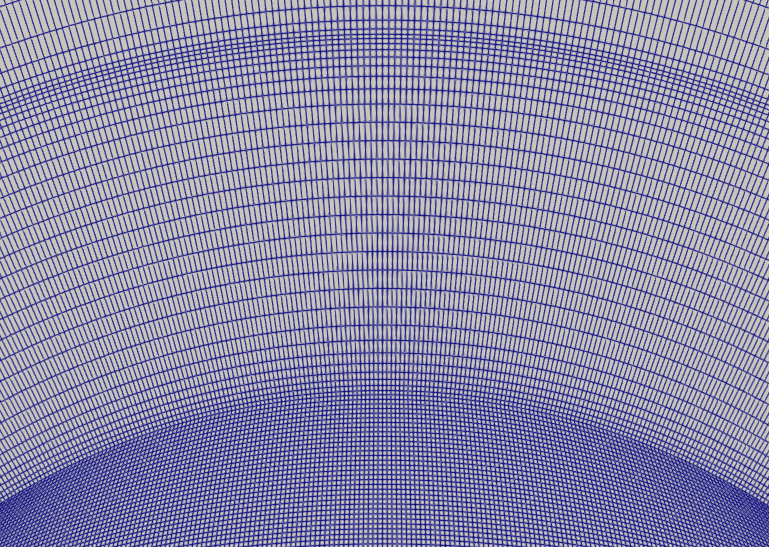
\includegraphics[width=0.4\textwidth]{images/numericalPump/diffuseurMesh.png}
    \caption{diffuseur Mesh}
    \label{diffuseurMesh}
\end{figure}

\begin{figure}[H]
    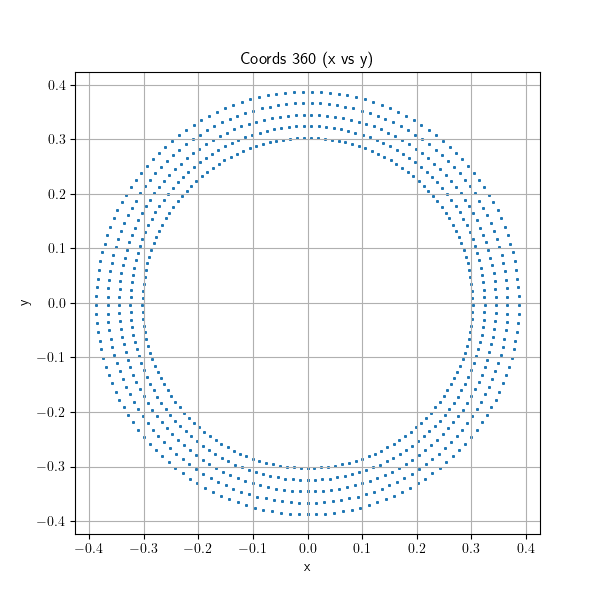
\includegraphics[width=0.4\textwidth]{images/coords360.png}
    \caption{Interpolation points over 360 degrees}
    \label{coords360}
\end{figure}

Limitations IBM à améliorer avec DA


\section{Application of the DA}

Explication de coords\_seventh.txt, coords\_360.txt et coords\_7.txt

Tentative d'explication en français :

J'ai d'un coté une simulation numérique de la pompe centrifuge, qui est un modèle numérique de la pompe. De l'autre coté, j'ai des données expérimentales de PIV, qui sont des données expérimentales de la pompe centrifuge. Je veux utiliser les données expérimentales pour améliorer le modèle numérique de la pompe centrifuge.
Pour cela, j'utilise la méthode de l'assimilation de données, qui est une méthode qui permet d'améliorer un modèle numérique en utilisant des données expérimentales. La méthode que j'utilise est l'Ensemble Kalman Filter (EnKF), qui est une méthode d'assimilation de données qui utilise un ensemble de modèles numériques pour améliorer le modèle numérique. 
Cela se fait en deux étapes :
\begin{enumerate}
    \item Je fais une simulation numérique de la pompe centrifuge, en utilisant le modèle numérique de la pompe centrifuge. Cette simulation numérique me donne un ensemble de modèles numériques, qui sont les membres de l'ensemble.
    \item Je compare les données expérimentales de PIV avec les données numériques de la simulation numérique. Pour cela, je fais une interpolation des données expérimentales de PIV sur les points de l'ensemble de modèles numériques. Cette interpolation me donne un ensemble de données expérimentales, qui sont les observations.
\end{enumerate}

La comparaison entre les données expérimentales et les données numériques me permet de calculer l'écart entre les deux, qui est appelé l'innovation (mettre référence partie mathématique). L'innovation est utilisée pour mettre à jour les membres de l'ensemble de modèles numériques, en utilisant la méthode de l'EnKF. Cette mise à jour me permet d'améliorer le modèle numérique de la pompe centrifuge.

1. Ma simulation numérique de la pompe est stationaire en utilisant la méthode MRF. Cela signifie que le champ de vitesse est constant dans le temps. Cepandant, il n'est pas constant dans l'espace, car il dépend de la position dans le diffuseur. Un motif de vitesse répété sept fois est donc censé être visible (cela n'est pas vraiment le cas en instantionnaire).

2. Les données PIV sont acquises à une vitesse de rotation de la pompe et une fréquence telle que 49 images sont acquises par tour de roue, soit 7 immages entre deux passage d'aubes successives. Dans le référentiel de la pompe, les images sont prises à un une différence de 360/49deg. 

Nous voulons comparer des données consitantes. Nous pourrions syncroniser une simulation instationnaire avec les données PIV. Mais nous avons choisis de faire une simulatio instationnaire dans un premier temps.

Nous pourrions reconstruire le champ spatial PIV (nous avons assez d'angle de vue et de données pour cale -> ref article Antoine).
Cependant, la vitesse de rotation n'est pas très précise, mais surtout, la méthode MRF inverse la forme du sillage.

Nous avons donc choisis de moyenner temporellement les données PIV (ce qui reviens à moyenner spatialement).
Du coté de la simulation, nous avons donc besoin de moyenner azimutalement les données numériques pour les rendre compatibles avec les données PIV.

\begin{figure}[H]
    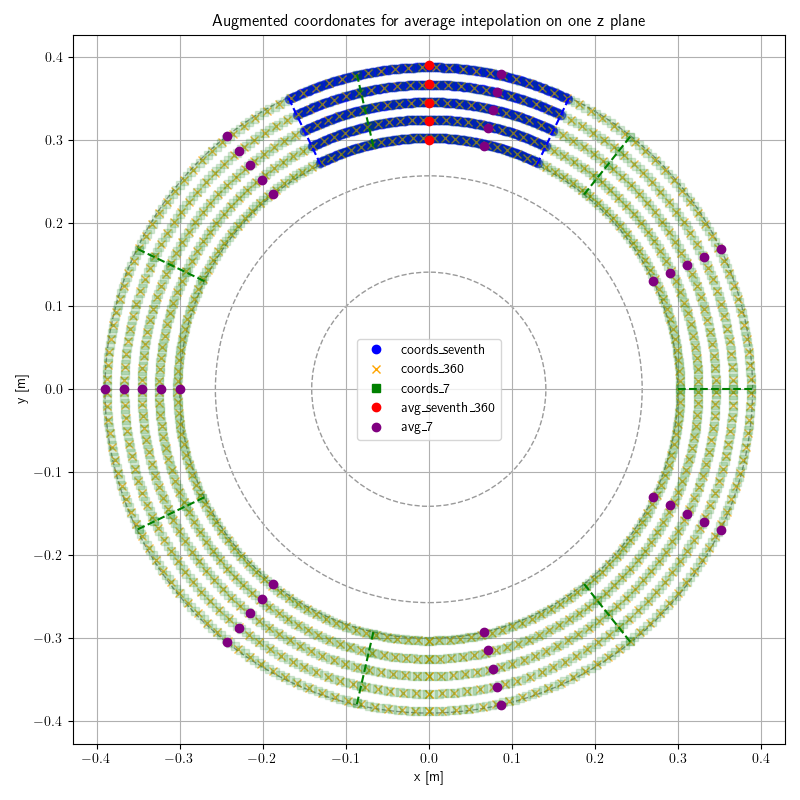
\includegraphics[width=0.8\textwidth]{images/numericalPump/coords.png}
    \caption{}
    \label{CHANGER}
\end{figure}

Imager avec des illustrations et vue en coupe ParaView

Pour cela j'ai commencé en moyennant 1/7 mais les paramètres étant locaux (non globaux), j'ai ensuite moyenné sur 360 degrés, ce qui permet de mieux prendre en compte les variations locales des paramètres. Cependant, nous pouvons converger vers une moyenne physique qui atteinds un minimum local mais qui ne respecte pas d'avoir 7 fois le même pattern. Cela permet à Fx d'être très différent de Fy mais aussi à la simulation de diverger avec des paramètres et vitesses erronéees. Pour palier ce problème, je compare la moyenne des patternes sur mes 7 segments de 360/7 degrés.





%S'aider du plan de la présentation MALEAF + thèse M

%Expliquer comment j'applique la DA sur le cas test de la pompe centrifuge (pas d'equation)

Nous avons fait l'EnKF sans l'état\dots
Sans inflation pour commencer. Si on converge vers une solution qui ne nous satisfait pas, on peut essayer d'ajouter... Cela permet de s'échaper d'un minimum local en ajoutant du bruit artificiellement. 

Nous avons fait une simu RANS mais nous aurion pu faire une simu URANS (ou LES ou DDES) avec un modèle de turbulence... 

L'expérience montre un ordre de grandeur de centaines d'itération entre les phases d'analyse, mais cela dépend beaucoup du cas.
Il en est de même pour le nombre de phases d'analyse.
Supposons 1000 itération en moyenne entre chaque phase d'analyse, et 300 phases d'analyse, cela nous fait 300 000 itérations à simuler, soit 93h, sur env. 2800 coeurs, soit 264kh.processeur de calcul.

Comment calculer la variance que je veux mettre ?
Expérience : 5\%
De mon coté : je vise qu'en moyenne un membre d'ensemble ait un écart de 1e7 par rapport au temps précédent (pour des valeurs autour de 5e7), donc, pour 30 membres d'ensemble, environ 95\% = 2 sigma dans 5e7+-1e7, càd sigma = 0.5e7 = 10\%. Ensuite, le nombre d'itération entre les phases d'analyse est déterminé en regardans combien d'itération sont nécessaires pour faire varier la solution dans le diffuseur (influe, rapidement, converge doucement mais ce qui nous intéresse c'est que ça prenne la tendace) lorsqu'un paramètre de forcage est modifié (supposé très inférieure pour la turbulence car appliquée de partout)

The observation window was defined by observing the number of iterations required for the influence of the IBM to reach the diffuser and take the form of the converged result. We are not interested in the turbulence parameters to determine the observation window because they are present throughout the domain, their influence is almost direct (not necessarily their convergence). We chose 800 iterations


Pb de la DA : plus rapide que DNS mais toujours plus lent que RANS et le temps d'attente et de calcul sur supercalculateur (sur 4000 processeurs) est de l'orde de plusieurs jours. On peut donc se demander si la DA est vraiment utile dans ce cas. En effet, la DA est plus rapide que la DNS mais pas que la RANS. Cependant, il faut prendre en compte le fait que la DA permet de réduire le temps de calcul de la simulation numérique en permettant d'optimiser les paramètres de l'IBM. De plus, la DA peut être utilisée pour d'autres cas d'étude où la DNS est trop coûteuse.



Pb perso : jusqu'à plusieurs jours d'attente pour lancer une simu.
%\begin{figure}[H]
%    \centering
%    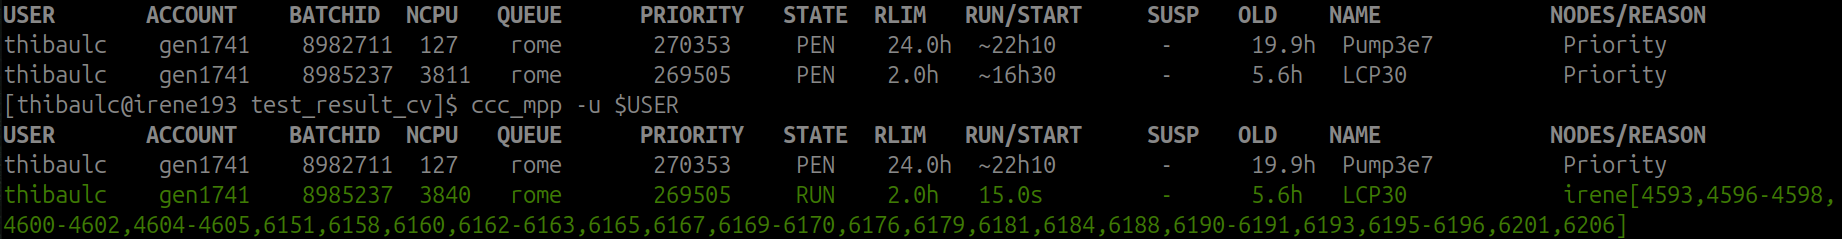
\includegraphics[width=0.5\textwidth]{images/other/queue_IRENE.png}
%    \caption{IRENE queue}
%    \label{queue_IRENE}
%\end{figure}

\subsection{Preprocessing of PIV data}

\subparagraph{Zone d'acquisition PIV}
\phantom{-}

The PIV data is acquired in a rectangular zone of 0.08 m x 0.124 m.
The cathesian coordinates are given in a local system, where the absolute origin is at the center of the pump.


\begin{figure}[H]
    \centering
    \begin{tikzpicture}
        \begin{axis}[
            axis equal,
            xlabel={$x$ (m)},
            ylabel={$y$ (m)},
            width=8cm,
            height=12cm,
            grid=both,
            xmin=0, xmax=0.08,
            ymin=0, ymax=0.124,
            title={Zone d'acquisition PIV}
        ]
        \draw[red, very thick, dashed] (0.0245, 0) -- (0.0245, 0.124);
        \node[red, rotate=90] at (0.053-0.031, 0.062) {$\theta = x_{abs} = 0$};


        % CentreAbs : (0,0)    -> CentreRel : (-0.0245,0.257.5)
        % BoutRel   : (0.06, 0.12) -> boutAbs : ...

        \draw[darkblue, very thick, dashed] (0.037756, 0) -- (0.0445, 0.124);
        \draw[darkblue, very thick, dashed] (0.051012, 0) -- (0.0645, 0.124);
        %\draw[darkblue, very thick, dashed] (0.02*(0.2575/0.3855)+0.0245, 0) -- (0.0245+0.02, 0.124);
        %\node[darkblue, rotate=90] at (0.053-0.031, 0.062) {$\theta = x_{abs} = 0$};
        
        \draw[->, >=stealth, color=darkblue, thick] (0.0245, 0.0145) -- (0.07-0.031, 0.0145);
        \node[darkblue, rotate=0] at (0.062-0.031, 0.017) {$\vec{x}$}; % _{abs}

        \draw[->, >=stealth, color=darkblue, thick]  (0.0245, 0.0145) -- (0.0245, 2*0.0145);
        \node[darkblue, rotate=0] at (0.021, 0.0195) {$\vec{y}$}; %_{abs}

        \draw[->, >=stealth, color=red, thick]  (0.0245, 0.1) -- (0.0245, 0.1145);
        \node[red, rotate=0] at (0.062-0.032, 0.108) {$\vec{U_{r}}$};

        \draw[->, >=stealth, color=red, thick]  (0.0245, 0.1) -- (0.01, 0.1);
        \node[red, rotate=0] at (0.0245-0.01, 0.1-0.005) {$\vec{U_{\theta}}$};


        \addplot+[
            only marks,
            mark=*,
            mark size=0.3pt,
            color=blue
        ] table [x index=0, y index=1] {autre/points_piv_tikz.txt};
        \end{axis}
    \end{tikzpicture}
\end{figure}

Dans la simulation numérique, l'axe z est vers le centre de la Terre, contrairement à l'expérience où il est vers le haut.
La roue tourne dans le sens trigonométrique dans le repère de la simulation numérique et dans le sens antitrigonométrique dans l'expérimentation.
Actuellement, je respecte le formalisme de la simu num pour le repère.

Parler des coefficients de relaxation.

\subparagraph{1.}

First, we need to know how to convert the coordinates from the local system to the absolute system.
We find that between the line 55 and 56, the radius is constant and pass from lower than \(\pi\) to upper. In fact, for the plan at 75\%, it is the same approache but between the line 65 and 66 because of some technical experimental constraints.
We also did plot x over theta for three differents values of theta and find out an intersection point for x = 0.0245.
So now, we know that for x = 0.0245, theta = \(\frac{\pi}{2}\)
%We could use the absolute system is defined by the following equations:
\begin{equation}
    \begin{cases}
        x_{rel} = x_{abs} + 0.0245 \\
        y_{rel} = x_{abs} + R_{2} \\ % R2 = 257.5
    \end{cases}
\end{equation}

\subparagraph{2.Average}
For now we are in stationary case (time invariant). So we are going to deal with data average over time.
There are around 49 maps (=file) by turn. So to agerage the data over the time, we can average over the \(\phi\) (\(\phi\) appartiens à 0-211rd) (=maps). That into the six directory.


\subparagraph{3.Sampling}
We will also average data between R1 and R2 to go to 3 files (of 10x81x125 elements).
Now, we keep only the data on the line x = 0.0245 (in fact we average data between x = 0.024 and x = 0.025). Data are then truncate at line 89, where the radius is upper than 0.3, because of some laser reflexion on the pump during the PIV experiment.


\subparagraph{4.Shaping for CONES}
Cones keep data in a particular way. We need to convert the data in a format that cones can read.
From 3 files (of 10x81x125 elements), to the files \texttt{fieldCylindrical.txt}
and \texttt{obs\_coordinates.txt}. Describe shapes...


\subparagraph{5.Creation of a file for the interpolation}
Finally, we need to create an \texttt{coords\_seventh.txt} file for the interpolation function in CONES.
We don't juste use the coordinates of the points in the PIV data, beacause we want to average over the angle \(\theta\) on the pump. The numerical simulation is $\frac{2\pi}{7}$ OU $2\pi/7$ periodic, so we interpolate in 150 points over theta between 0 and 2pi/7.
To do that, wue just take the \texttt{obs\_coordinates.txt} file and duplicate 150 times the points over the angle \(\theta\) (between -pi/7 and pi/7). In our case, we chose 150 that will aproximately correspont to the shap of a cell at this radius.
To be consistent with axis further, we take points between -pi/7 + pi/2 and pi/7 + pi/2

Here is the plot of the experimental data and the numerical data (for D = 3e7 (introduire la variable)), at the same points (both are averages over time and over the angle \(\theta\)).




potentiellement en annexe

Concretely, to average the data over the angle \(\theta\), we need to modify the interpolation function in CONES.
Instead of read coords, the interpolation function read the data in the \texttt{coords\_seventh.txt} file.

Then, it computes the interpolation and average the data over the angle \(\theta\) (between -pi/7 and pi/7), by doing a somme over \(\theta\) and dividing by the number of points (150). To go back from 150x5x3x3 (to detail) to 5x3x3 data. All of those computation are mad in a cylindrical referencial. Ref au schéma tikz


A sixth coefficients DP has been add.
It's represent the difference of pressure between the inlet of the pipe and the outlet of the diffuser. 
The numerical coefficient are interpolating, respectively at (0,0,-0.35) and (0,0.390,0).
For the high fidelity value, we can find experimental data form the same pump [M. Fan 2022], that's match with M. Fan simulation (eq to approximately \(\eta\) = 0.4). So can also compute :



U\_{2} is the impeller tip speed computed from the impeller diameter and the rotation speed of the pump.

\begin{equation}
    \frac{\Delta P_{P}}{\rho U_{2}^{2}} = \eta \Leftrightarrow
    \Delta P_{P} = \rho U_{2}^{2} \eta
\end{equation}

U2carré = (omega * R2)² = (2 * pi * 1200 / 60 * 0.2566)² = 32,2 m/s

As we are in a steady simulation, the restult of the numerical pressure is divided by the density of the fluid.

\begin{equation}
    \Delta P_{P} = 32.2^{2} \times 0.4 = 415 Pa
\end{equation}

So the state vector is now 46.
Incertitude on P will be less to take more take it account.
Inflation...

At pump flow rate = pump design flow rate So Q?/Q? =1

\subsection{Modifications on OpenFoam and CONES} %Preparation

Tout ce qu'il y a dans le CONES dict
Parler des modifs dans le code ici.



- Réduction du pipe (avec recherche condition vitesse entrée)




\section{Results}

Comparer les 3 résultats : avant DA, après simple et "complex" DA


\begin{figure}[H]
    \centering
    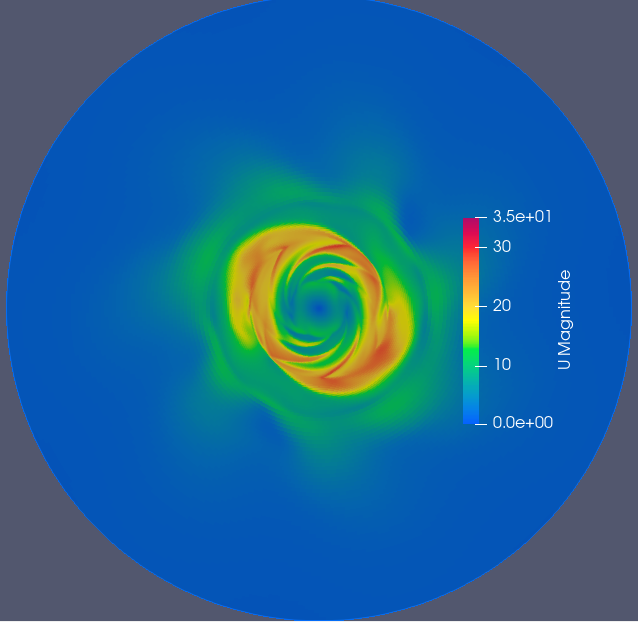
\includegraphics[width=0.5\textwidth]{images/numericalPump/assymetrie.png}
    \caption{Velocity field for Dx = 4e7 and Dy = 2e7}
    \label{fig:assymetry}
\end{figure}



\begin{figure}[H]
    \centering
    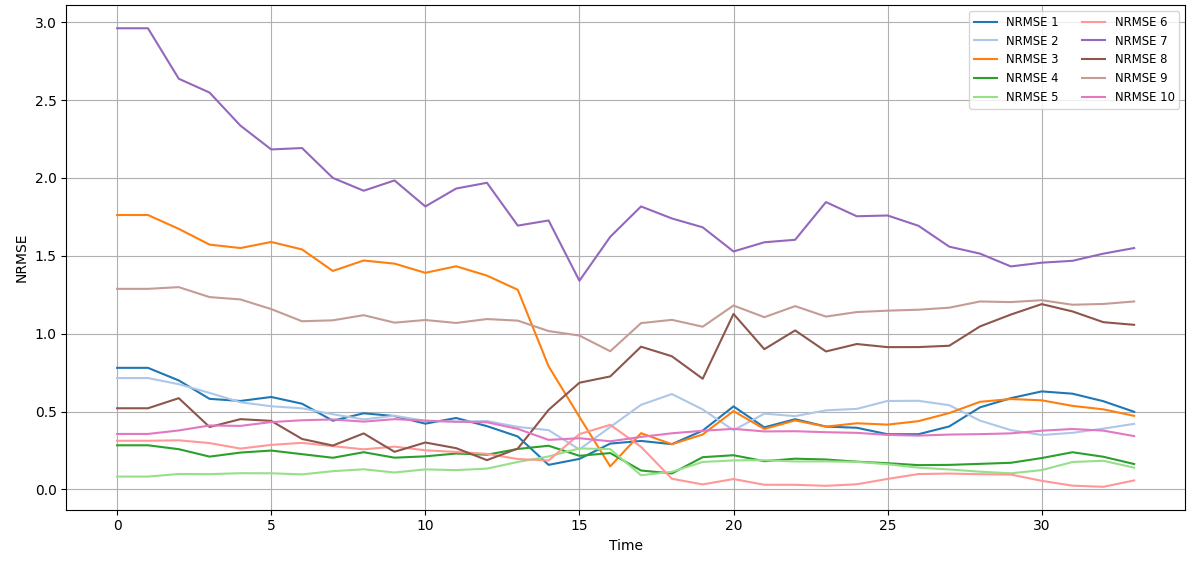
\includegraphics[width=0.5\textwidth]{images/UpdtC14_10NMRSE.png}
    \caption{Evolution of the NRMSEs over EnKF analysis phases}
    \label{fig:UpdtC14_10NMRSE}
\end{figure}


\dots

Explication des écarts par différentes choses 


Tt ce que j'ai implémenté en plus (déjà détaillé partie précédente normalement)

\begin{figure}[H]
    \centering
    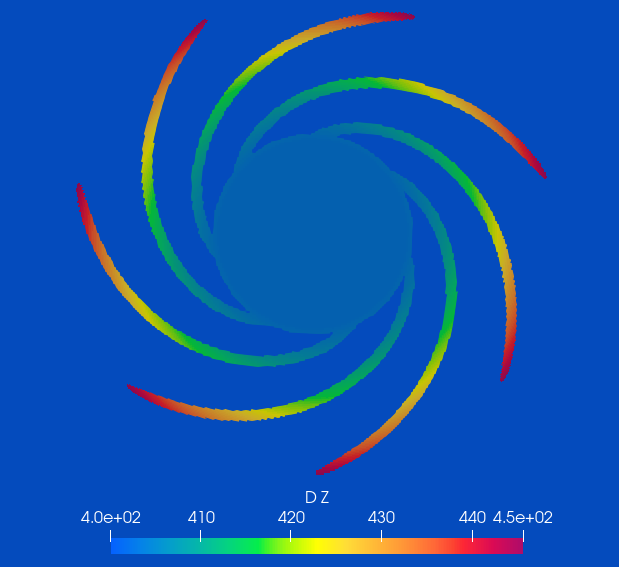
\includegraphics[width=0.5\textwidth]{images/numericalPump/radialExpension.png}
    \caption{Radial expension of Dz over the impeller radius}
    \label{fig:radialExpension}
\end{figure}



Essayer d'améliorer le rendu de l'image ci-dessous en mettant la pompe en transparence
\begin{figure}[H]
    \centering
    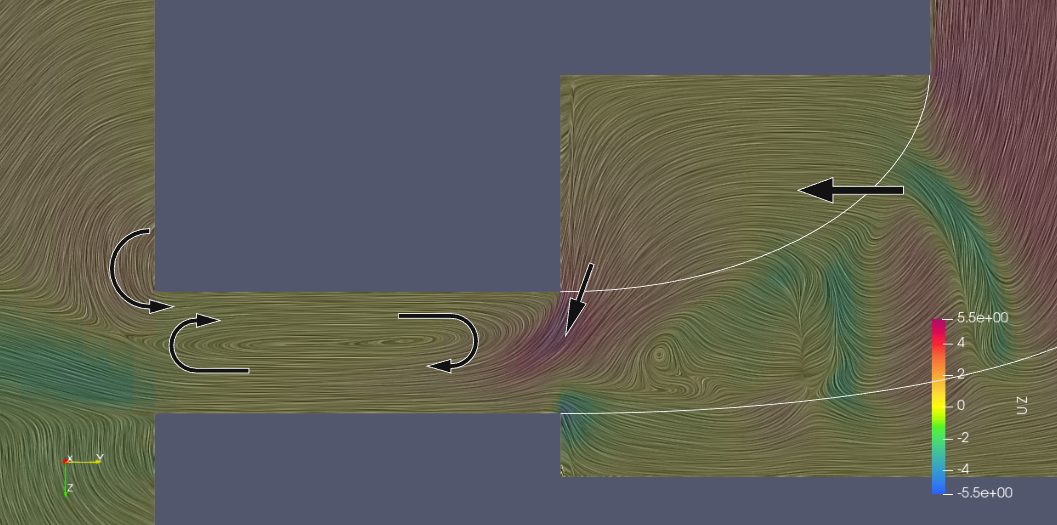
\includegraphics[width=0.5\textwidth]{images/numericalPump/LIC.png}
    \caption{Formation of the recirculation bubble in the diffuser}
    \label{fig:LIC}
\end{figure}

Explication des écarts par la bulle de recirculation.

\subsection{Conclusion ans perspective}

Problème de méthode et pas de miracle ave cette méthode IBM. Interpolation, instationnaire (avantage : on ne contraint plus avec MRF et donc plus facile de réconcilier solution numérique physique et mathématique)


Ouverture : méthode IBM interpolation, article non référencé.

\cite{valeroEnhancedStateEstimation2025} -> ML turbulent channel flow Miguel

"Ouverture / idée" : DA temps réel dans avion impossible pour encore longtemps.
Solution : Contrôle actif de la puissance en fonction des mesures de pression dans le compresseur :
f(obs) -> controle de la puissance
Pour ça, se ref au sujet de thèse de Tarane
obs pression --> modèle de reconstruction du champ de vitesse --> modèle de reconaissance de patternes de décrochage --> contrôle de la puissance
Peut-être faire deux filtres de Kalman imbriqués ? hyperparamètres type fenetre observation, variance initiale, ...



Voir "TD -> Done et "TDSave -> Done" pour voir tt ce que j'ai fais


The random variations are random but with a reproducibility seed (sed) that allows to have the same result each time the simulation is launched.
